% \documentclass{article}
% \usepackage[utf8]{inputenc}
% \usepackage{listings}
% \usepackage{graphicx}
% \graphicspath{ {images/} }
% \lstset{language=XML}
%
% \title{Mobile programming- Laboratorio 3}
% \author{pasoa}
% \date{June 2017}

% \begin{document}

% \maketitle

\chapter{Addattarsi al cambiamento di configurazioni}
Quando si verifica un cambiamento nella configurazione, il sistema runtime di
Android fa ricominciare le attività e i fragment. Questo accade per dare la
possibilità all'applicazione di adattarsi all'ambiente con la nuova
configurazione, rilanciandola automaticamente. Troviamo diversi tipi di eventi
che generano questa operazione, come ad esempio il cambio dell'orientamento
dello schermo.\\
Il riferimento lo troviamo in \texttt{android:configChange}.\\
Chiaramente questo fenomeno, se non gestito, ha conseguenze catastrofiche: tutte
le variabili delle nostre attività e frammenti verranno distrutte e ricaricate,
perdendo di conseguenza le informazioni su cui si stava lavorando. È necessario
così salvare lo stato del processo prima che le attività (o frammenti) vengano
ditrutte e caricare tale stato al verificarsi di
\texttt{(onSave(Restore)InstanceState())}; tuttavia interrompere un processo in
esecuzione può essere indesiderato o costoso.\\
Dobbiamo infatti tener conto che l'esecuzione di operazioni quali
\texttt{onSaveInstanceState} e \texttt{onReloadInstanceState} possono arrecare
una sgradevole esperienza per l'utente (per la complessità delle operazioni) ed
inoltre potrebbe non essere possibile ripristinare completamente lo stato
dell'activity con il \textit{Bundle}: questa operazione di ripristino non è
realizzabile per grossi oggetti ed i dati devono essere serializzati e
deserializzati.\\
In queste situazioni possiamo pensare di dover gestire il cambiamento di
configurazione noi stessi oppure conservare un oggetto durante tale evento.
\subsection{Impedire il riavvio del sistema}
Vogliamo impedire il riavvio del sistema al cambiamento di una configurazione.
Possiamo gestire il il cambiamento manualmente con la funzione 
\texttt{onConfigurationChanged}. A tale metodo passiamo un \textit{oggetto di
configurazione} nel quale sono specificate le configurazioni del nuovo device.
Quando esso viene chiamato l'\textit{oggetto Resource} viene aggiornato con la
nuova configurazione.\\
Nel file \textit{manifest.xml} dobbiamo quindi specificare quali sono i
cambiamenti che gestiamo:
\begin{lstlisting}[frame=single]  % Start your code-block
<activity android:name=".MyActivity"
 android:configChanges="orientation|keyboardHidden"
 android:label="@string/app_name">
\end{lstlisting}
Quindi, in questo caso, stiamo dicendo che il sistema non si riavvierà al
verificarsi di \textit{orientation} e \textit{keyboardHidden} ma saremo noi a
gestirli.
Nella Activity gestiremo il tutto come segue:

\begin{lstlisting}[frame=single]  % Start your code-block

@Override
public void onConfigurationChanged
    (Configuration newConfig) {
 super.onConfigurationChanged(newConfig);



 // Checks the orientation of the screen
 if (newConfig.orientation ==
    Configuration.ORIENTATION_LANDSCAPE) {
 Toast.makeText(this, "landscape",
    Toast.LENGTH_SHORT).show();
 } else if (newConfig.orientation ==
    Configuration.ORIENTATION_PORTRAIT){
 Toast.makeText(this, "portrait",
    Toast.LENGTH_SHORT).show();
 }
}
\end{lstlisting}
In questo modo possiamo decidere noi come gestire il tutto.

\subsection{Conservare l'oggetto durante il cambiamento}
Questa è la scelta raccomandata. Questa procedura permette il riavvio alla 
Activity al generarsi di un cambiamento di configurazione, ma tiene un oggetto
con lo stato per la nuova istanza. Per mantenere lo stato durante il 
cambiamento è possibile utilizzare una \textit{Fragment class}.
Gli step da seguire sono i seguenti:
\begin{itemize}
    \item estendere la Fragment class e dichiarare i riferimenti all'oggetto
    \item quando il frammento è creato chiamare
\textit{setRetainInstance(boolean)}
    \item aggiungere il frammento all'activity
    \item usare il \textit{fragment manager} per recuperare il frammento al
riavvio dell'activity
\end{itemize}
Ad esempio:
\begin{lstlisting}[frame=single]
public class RetainedFragment extends Fragment {

 // data object we want to retain
 private MyDataObject data;



 // this method is only called once for this fragment
 @Override
 public void onCreate(Bundle savedInstanceState) {
 super.onCreate(savedInstanceState);
 // retain this fragment
 setRetainInstance(true); }
 }
 @Override
 public void onAttach(Context context) {
 //called when Activity:onCreate() has finnished
 //update the pointer to the activity: (Activity)context
 }
}
\end{lstlisting}
\section{Datastorage in Android}
Possiamo salvare un semplice file come sequenza di dati. Il salvataggio può 
essere fatto in due posizioni:
\begin{itemize}
    \item \textit{Internal Storage}: possiamo salvare il file direttamente nella
memoria interna ed il file salvato sarà privato, ovvero accessibile solo
dall'applicazione (altre applicazioni non possono accedervi)
    \item \textit{External Storage}: possiamo salvare il file in una memoria
esterna, come ad esempio una SD card, oppure nella memoria del telefono; con
questo tipo di configurazione il file sarà accessibile da altre applicazioni
\end{itemize}
Possiamo salvare in insiemi Chiave-Valore: utilizziamo un \textit{shared
preference file} il quale ci permette di svolgere questa operazione. In questo
caso i dati persistono anche se l'applicazione viene chiusa. \\
Un'altra soluzine consiste nell'uso di \textit{SQLite Database}, ovvero una
struttura per il salvataggio di informazioni in un database; Android memorizza
il database in uno spazio privato non accessibile da altre applicazioni.
\subsubsection{SQLite DB}
È una libreria che ci permette di gestire un database senza l'utilizzo di un
server. Essa comprende tutte le funzionalità dei database e supporta alcuni
tipi di dato, come INTEGER, REAL, TEXT. Prima di memorizzare i nostri dati sul
database, dobbiamo convertirli in tali tipi.\\
La classe \texttt{SQLite Manager} ci permette di gestire il database. In essa
dobbiamo definire le componenti del database, come il nome, le tabelle con i
relativi campi e le query. Troviamo override di metodi quali \texttt{onCreate},
chiamato alla creazione del database, e \texttt{onUpgrade} per aggiornarne la
versione, stabilendo il modo in cui farlo e cosa farne nei dati precedentemente
salvati.\\
Operazioni comuni in un database sono la lettura e scrittura; per farlo dobbiamo
avere un riferimento al database. Per inserire dati passiamo tramite l'oggetto
\texttt{ContentValues}, il quale accetta una coppia chiave-valore, ad esempio:
\begin{lstlisting}[frame=single]
ContentValues values = new ContentValues();
values.put(MySQLiteHelper.COLUMN_NAME, value);
\end{lstlisting}
Per la lettura utilizziamo un oggetto \texttt{Cursor}, che conterrà il risultato
della ricerca; ad esempio:
\begin{lstlisting}[frame=single]
Cursor cursor = database.query(
    MySQLiteHelper.TABLE_CONTACTS, /* name of table */
    allColumns, /* projection: all columns */
    MySQLiteHelper.COLUMN_ID + /* selection: where
                                    clause */
    " = " + insertId, /* this particular id */
    null, /* don't use selection args */
    null, /* don't group the rows */
    null, /* don't filter by row groups */
    null); /* don't sort the order */
\end{lstlisting}
Per leggere una riga del risultato contenuto nel Cursor dobbiamo prima settarne
la posizione di inizio (e.g. cursor.MoveToFirst() per iniziare dal primo
elemento, cursor.MoveNext() per passare all'elemento successivo a quello
attuale, ...).\\
Per eliminare il database, possiamo utilizzare il metodo di database helper
\texttt{delete} dove specifichiamo cosa vogliamo eliminare.
\begin{lstlisting}[frame=single]
database.delete(MySQLiteHelper.TABLE_CONTACTS,
MySQLiteHelper.COLUMN_ID   + " = " + id, null);
\end{lstlisting}
È importante gestire correttamente l'acquisizione e il rilascio delle risorse
durante la vita dell'attività:
\begin{lstlisting}[frame=single]
@Override
 protected void onResume() {
 datasource.open();
 super.onResume();
 }

 @Override
 protected void onPause() {
 datasource.close();
 super.onPause();
 }
\end{lstlisting}
Lettura e scrittura su database provocano un consumo maggiore di prestazioni e 
l'esperienza utente potrebbe risentirne. Per risolvere questo problema Android
mette a disposizione letture asincrona chiamate \texttt{CursorLoader} e
\texttt{AsyncTaskLoader}\textit{--}\texttt{LoadingInBackground()}. Il cursor
Loader richiede un implementazione del \textit{Content Provider}.
\section{Content Provider}
L'obiettivo del content provider è quello di gestire l'accesso ai dati e
fornirne meccanismi per la definizione della loro sicurezza. Come accennato in
precedenza, il \textit{CursorLoader} fa affidamento al content provider per
l'esecuzione di query asincrone per poi ritornare il risultato alla UI.
\begin{figure}
    \centering
    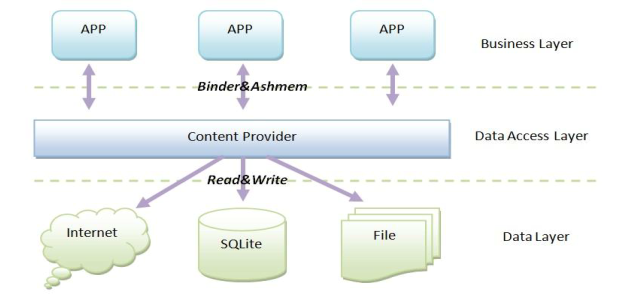
\includegraphics[scale = 0.6]{cp}
    \caption{Content Provider}
    \label{fig:my_label}
\end{figure}
Il suo comportamento è simile ai database in quanto possiamo fare domande
(query), modificarne il contenuto, inserire, eliminare ed aggiornare i dati.
Nella maggior parte dei casi il contenuto è memorizzato in database SQLite. \\
Le query al content provider vanno definite in un formato
specifico (URI):\\$<prefix>://<authority>/<data\_type>/<id>$\\
dove:
\begin{itemize}
    \item prefisso: sempre impostato sul contenuto
    \item authority: specifica il nome del content provider
    \item data\_type: indica il tipo di dati che il provider fornisce
    \item id: indica la specifica riga da richiedere
\end{itemize}
Ad esempio, se volessimo avere informazioni per il quinto contatto del content
provider "Content" l'URI sarà del tipo: \texttt{content://contacts/people/5}
dove \textit{people} è il tipo di dato che ci ritorna.\\
Per creare una classe Content Provider come prima cosa dobbiamo estendere
\texttt{ContentProvider}; dopodiché dobbiamo definire l'URI, il quale verrà
usato per accedere ai contenuti. Dobbiamo inoltre definire il database (usando
SQLite) che conterrà le informazioni; a questo punto si definiscono le
possibili queries per specifiche operazioni. Infine, registriamo il Content
Provider nell'activity tramite il tag "\texttt{<provider>}".\\
I principali metodi che dobbiamo sovrascrivere sono:
\begin{itemize}
    \item onCreate(): chiamato alla creazione del provider
    \item query(): riceve una richiesta dal client; il risultato è ritornato in
un oggetto Cursor
    \item insert(): inserisce un nuovo record nel content provider
    \item delete(): elimina un record dal content provider
    \item update(): aggiorna un record esistente
    \item getType(): ritorna il tipo di dato dato un URI
\end{itemize}
% \end{document}
